% Provenance (never printed): cycle 4 SVT, "La planete Terre": volcanic
% activity, its products and its link with plate boundaries; natural hazards
% and their monitoring; see sources/book1/PROVENANCE.md. Book 1, grade 7,
% chapter 2.
% Vocabulary guard: "magma" first allowed here; "sediment" not before g7.4;
% "subduction zone" is never a term here (gloss: "where one plate sinks under
% another"); "hotspot track" is Book 2's; lahars are called mudflows.
\chapter{ज्वालामुखी}\label{ch:g7:volcanoes}

17~मई 1980 को एक भूवैज्ञानिक संयुक्त राज्य अमेरिका के उत्तर-पश्चिम में माउंट
सेंट~हेलेंस से दस किलोमीटर दूर एक \omterm{def:g1:landscapes-around-us:landform}{पहाड़ी} कटक पर खड़ा था, और उसने नीचे बाईं ओर
वाली तस्वीर ली: बर्फ़ से ढका एक चिकना शंकु, देश के सबसे सुंदर पहाड़ों में से एक।
दो महीनों से पहाड़ काँप रहा था, और उसका उत्तरी हिस्सा एक गुब्बारे की तरह बाहर
की ओर फूल रहा था। अगली सुबह 8:32 बजे एक छोटे \omterm{def:g4:volcanoes-earthquakes-first-look:earthquake}{भूकंप} ने उसे हिला दिया। फूला हुआ
पूरा हिस्सा फिसलकर नीचे चला गया, और \omterm{def:g4:volcanoes-earthquakes-first-look:volcano}{ज्वालामुखी} एक तरफ़ को फट पड़ा। जब सितंबर
में उसी कटक से फिर तस्वीर ली जा सकी, तो पहाड़ दाईं ओर वाली तस्वीर जैसा
दिखता था।

\begin{omfigure}
\begin{minipage}[b]{0.495\linewidth}\centering
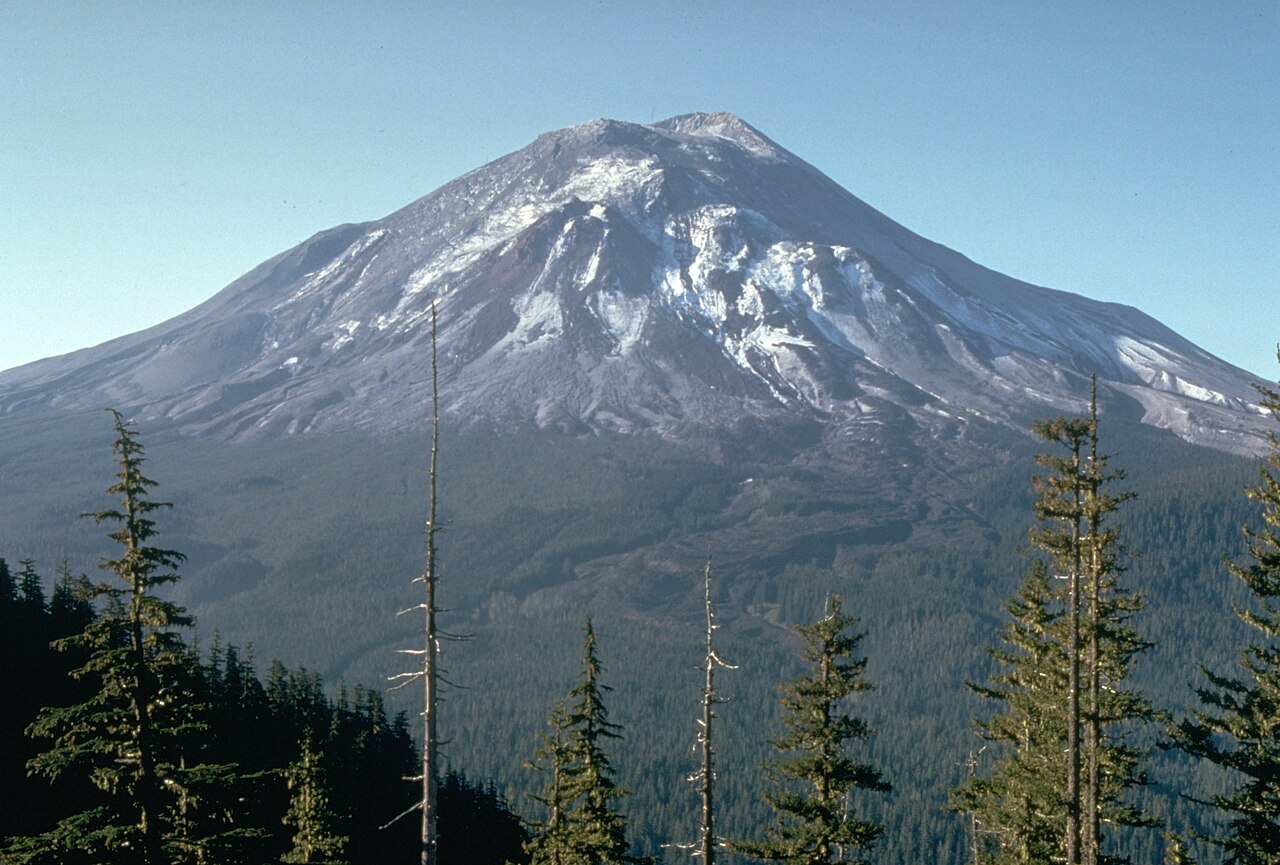
\includegraphics[width=\linewidth]{images/book1/g7-msh-before.jpg}

{\small 17 मई 1980, एक दिन पहले।}
\end{minipage}\hfill
\begin{minipage}[b]{0.495\linewidth}\centering
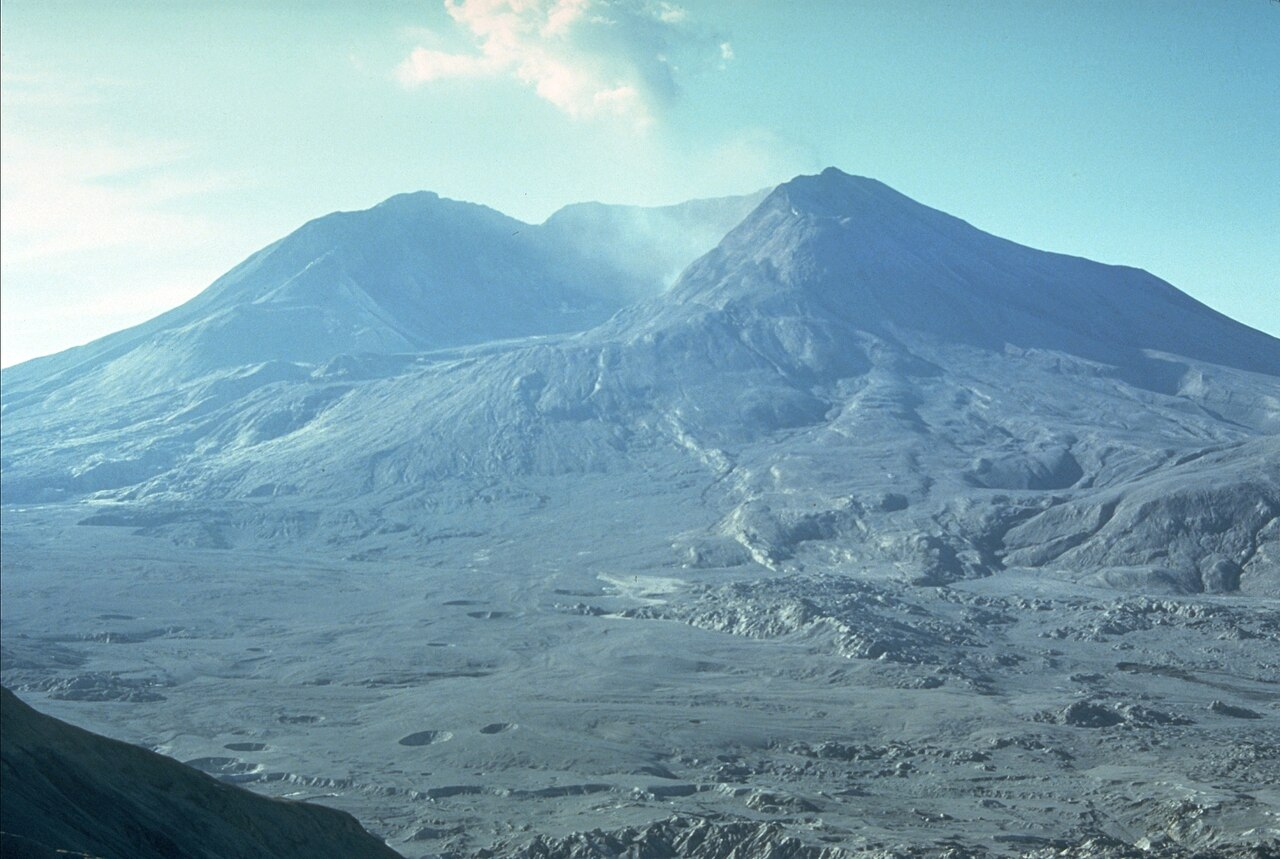
\includegraphics[width=\linewidth]{images/book1/g7-msh-after.jpg}

{\small 10 सितंबर 1980।}
\end{minipage}

{\small जॉनस्टन रिज से दिखता माउंट सेंट~हेलेंस, 18~मई 1980 के \omterm{def:g4:volcanoes-earthquakes-first-look:eruption}{उद्गार} से पहले और
बाद। चोटी और पूरा उत्तरी हिस्सा ग़ायब है; उनकी जगह उत्तर की ओर खुला एक \omterm{def:g7:volcanoes:vent}{क्रेटर}
है। फ़ोटो: हैरी ग्लिकेन, अमेरिकी भूवैज्ञानिक सर्वेक्षण (सार्वजनिक डोमेन,
विकिमीडिया कॉमन्स के ज़रिए)।}
% ledger: commons:msh-before, commons:msh-after, usgs:msh-lead-up, usgs:msh-may18
\label{fig:g7:volcanoes:st-helens}
\end{omfigure}

इस अध्याय में हम एक \omterm{def:g4:volcanoes-earthquakes-first-look:volcano}{ज्वालामुखी} को खोलकर देखेंगे कि \omterm{def:g4:volcanoes-earthquakes-first-look:eruption}{उद्गार} को क्या चलाता है;
पता करेंगे कि कुछ \omterm{def:g4:volcanoes-earthquakes-first-look:volcano}{ज्वालामुखी} \omterm{def:g4:volcanoes-earthquakes-first-look:eruption}{लावा} की शांत \omterm{def:g1:landscapes-around-us:water}{नदियाँ} क्यों बहाते हैं जबकि दूसरे खुद
को उड़ा देते हैं; और \omterm{def:g3:continents-and-oceans:world-map}{विश्व मानचित्र} को फिर देखेंगे, यह जानने के लिए कि
\omterm{def:g4:volcanoes-earthquakes-first-look:volcano}{ज्वालामुखी} कहाँ हैं और क्यों।

\begin{recall}
\emph{\omterm{def:g4:volcanoes-earthquakes-first-look:volcano}{ज्वालामुखी}} वह जगह है जहाँ पृथ्वी के भीतर गहरे से पिघली \omterm{def:g3:stones-pebbles-sand:rock}{चट्टान} सतह पर
बाहर आती है, और वह \omterm{def:g1:landscapes-around-us:landform}{पहाड़ी} या पहाड़ भी जो वह वहाँ बनाती है। \emph{\omterm{def:g4:volcanoes-earthquakes-first-look:eruption}{उद्गार}} के
दौरान वह \omterm{def:g4:volcanoes-earthquakes-first-look:eruption}{लावा}, राख और गैस बाहर फेंकता है
(\cref{ch:g4:volcanoes-earthquakes-first-look})। \omterm{def:g6:inside-the-earth:layers}{भूपर्पटी} के नीचे \omterm{def:g6:inside-the-earth:layers}{प्रावार} गरम
\omterm{def:g3:stones-pebbles-sand:rock}{चट्टान} का बना है जो ठोस है, हालाँकि वह बहुत धीरे-धीरे सरक सकती है
(\cref{ch:g6:inside-the-earth})। बेसाल्ट और ग्रेनाइट \omterm{def:g6:rocks-and-minerals:rock-families}{आग्नेय चट्टानें} हैं: वे
तब बनती हैं जब पिघली \omterm{def:g3:stones-pebbles-sand:rock}{चट्टान} ठंडी होकर सख़्त हो जाती है
(\cref{ch:g6:rocks-and-minerals})। पृथ्वी का बाहरी कवच \omterm{def:g7:plate-tectonics:plate}{प्लेटों} में टूटा है जो
साल में कुछ सेंटीमीटर चलती हैं; उनके किनारे \omterm{def:g7:plate-tectonics:plate-boundary}{प्लेट सीमाएँ} हैं
(\cref{ch:g7:plate-tectonics})।
\end{recall}

\section{ज्वालामुखी के अंदर}

\omterm{def:g6:inside-the-earth:layers}{प्रावार} ठोस है। फिर भी कुछ जगहों पर, सतह के बहुत नीचे, \omterm{def:g3:stones-pebbles-sand:rock}{चट्टान} का एक छोटा
हिस्सा पिघल जाता है। पिघली \omterm{def:g3:stones-pebbles-sand:rock}{चट्टान} अपने आसपास की ठोस \omterm{def:g3:stones-pebbles-sand:rock}{चट्टान} से हल्की होती है,
इसलिए वह धीरे-धीरे ऊपर उठती है, दरारों में से रास्ता बनाते हुए, जैसे पानी में
से तेल की एक बूँद ऊपर उठती है।
% ledger: usgs:hawaii-hotspot (magma lighter than the surrounding rock, rises)

\begin{definition}[मैग्मा]\label{def:g7:volcanoes:magma}
\emph{मैग्मा}\index{मैग्मा} ज़मीन के नीचे की पिघली \omterm{def:g3:stones-pebbles-sand:rock}{चट्टान} है। यह एक गरम द्रव
है जिसमें क्रिस्टल भी हो सकते हैं और जिसमें जलवाष्प और कार्बन डाइऑक्साइड जैसी
गैसें घुली होती हैं। जो मैग्मा सतह पर बाहर आता है, उसे \omterm{def:g4:volcanoes-earthquakes-first-look:eruption}{लावा} कहते हैं; बाहर
आते समय वह अपनी ज़्यादातर गैस खो देता है।
\end{definition}

ऊपर उठता \omterm{def:g7:volcanoes:magma}{मैग्मा} अक्सर रास्ते में, सतह से कुछ किलोमीटर नीचे, रुक जाता है, जहाँ
वह एक बड़ी जेब में जमा हो जाता है। वहाँ वह इंतज़ार करता है, कभी-कभी सदियों तक,
इससे पहले कि कोई \omterm{def:g4:volcanoes-earthquakes-first-look:eruption}{उद्गार} उसका एक हिस्सा ख़ाली कर दे।

\begin{definition}[मैग्मा कक्ष]\label{def:g7:volcanoes:magma-chamber}
\emph{मैग्मा कक्ष}\index{मैग्मा कक्ष} किसी \omterm{def:g4:volcanoes-earthquakes-first-look:volcano}{ज्वालामुखी} के नीचे, कुछ किलोमीटर
गहराई पर, \omterm{def:g3:stones-pebbles-sand:rock}{चट्टानों} में एक बड़ी जगह है जहाँ \omterm{def:g4:volcanoes-earthquakes-first-look:eruption}{उद्गार} से पहले \omterm{def:g7:volcanoes:magma}{मैग्मा} जमा
होता है।
\end{definition}

\begin{definition}[निकास-छिद्र और क्रेटर]\label{def:g7:volcanoes:vent}
\emph{निकास-छिद्र}\index{निकास-छिद्र} सतह पर एक मुँह है जिससे \omterm{def:g7:volcanoes:magma}{मैग्मा}, गैस और
राख बाहर आते हैं। \emph{क्रेटर}\index{क्रेटर} किसी निकास-छिद्र के चारों ओर का
कटोरे के आकार का गड्ढा है, जो आमतौर पर \omterm{def:g4:volcanoes-earthquakes-first-look:volcano}{ज्वालामुखी} की चोटी पर होता है।
\end{definition}

\begin{omfigure}
\begin{tikzpicture}[font=\small, x=1cm, y=1cm]
  % rocks below the volcano
  \fill[brown!25] (-6,-4.2) rectangle (6,0);
  \draw[brown!50] (-6,-1.4) -- (6,-1.4) (-6,-2.8) -- (6,-2.8);
  % the cone, built of layers of lava (dark) and ash (light)
  \fill[black!45] (-5.2,0) -- (-0.75,3.4) -- (0.75,3.4) -- (5.2,0) -- cycle;
    % layers dipping outwards, parallel to the flanks (slope 3.4/4.45)
  \foreach \k/\c in {0/black!25, 2/black!25, 4/black!25} {
    \pgfmathsetmacro{\xa}{-5.2+0.8*\k}\pgfmathsetmacro{\xb}{-5.2+0.8*(\k+1)}
    \pgfmathsetmacro{\ya}{(-0.18-\xa)*3.4/4.45}\pgfmathsetmacro{\yb}{(-0.18-\xb)*3.4/4.45}
    \fill[\c] (\xa,0) -- (-0.18,\ya) -- (-0.18,\yb) -- (\xb,0) -- cycle;
    \fill[\c] (-\xa,0) -- (0.18,\ya) -- (0.18,\yb) -- (-\xb,0) -- cycle;
  }
  % the crater at the top
  \fill[white] (-0.75,3.4) -- (-0.3,2.95) -- (0.3,2.95) -- (0.75,3.4) -- cycle;
  \draw[black!70] (-0.75,3.4) -- (-0.3,2.95) -- (0.3,2.95) -- (0.75,3.4);
  % magma chamber and the pipe up to the vent
  \fill[orange!85!red] (0,-3.0) ellipse (2.1 and 0.75);
  \fill[orange!85!red] (-0.18,-2.4) rectangle (0.18,2.98);
  % a side branch to a small side vent
  \fill[orange!85!red] (0.1,0.6) -- (2.55,1.5) -- (2.62,1.33) -- (0.1,0.25) -- cycle;
  % lava flow down the right flank, from the side vent
  \fill[orange!95!red] (2.5,1.45) .. controls (3.2,1.0) and (3.7,0.5) .. (4.6,0.08)
    -- (4.0,0.05) .. controls (3.3,0.4) and (2.9,0.8) .. (2.45,1.25) -- cycle;
  % ash column and gas
    \fill[black!22] (-0.3,3.0) -- (0.3,3.0) -- (0.45,3.9) -- (-0.45,3.9) -- cycle;
  \foreach \x/\y/\r in {0/3.95/0.45, -0.45/4.55/0.55, 0.45/4.6/0.5, -0.15/5.2/0.6,
                        0.6/5.3/0.5, -0.8/5.15/0.45, 0.15/5.8/0.55}
    \fill[black!22] (\x,\y) circle (\r);
  % labels
  \node[anchor=west] at (2.1,5.3) {राख और गैस का स्तंभ};
  \draw[black!60] (2.05,5.3) -- (1.05,5.2);
  \node[anchor=west] at (2.0,3.3) {क्रेटर};
  \draw[black!60] (1.95,3.3) -- (0.6,3.2);
  \node[anchor=east] at (-2.0,3.8) {मुख्य निकास-छिद्र};
  \draw[black!60] (-1.95,3.75) -- (-0.1,3.0);
  \node[anchor=west] at (4.2,1.6) {पार्श्व निकास-छिद्र};
  \draw[black!60] (4.15,1.6) -- (2.65,1.45);
  \node[anchor=west] at (4.5,0.55) {लावा प्रवाह};
  \draw[black!60] (4.45,0.55) -- (3.9,0.4);
  \node[anchor=east, align=right] at (-3.0,1.75) {लावा और राख\\की परतें};
  \draw[black!60] (-2.95,1.6) -- (-2.2,1.1);
  \node[anchor=west, align=left] at (0.55,-0.9) {नली में ऊपर\\उठता मैग्मा};
  \draw[black!60] (0.5,-0.9) -- (0.2,-0.9);
  \node[anchor=west] at (2.3,-3.0) {मैग्मा कक्ष};
  \draw[black!60] (2.25,-3.0) -- (1.7,-3.0);
  \node[anchor=west, align=left, font=\footnotesize] at (-5.9,-3.7) {कुछ किलोमीटर नीचे};
  \draw[black!60, <->] (-4.3,0) -- (-4.3,-3.0);
\end{tikzpicture}

{\small खोलकर दिखाया गया एक \omterm{def:g4:volcanoes-earthquakes-first-look:volcano}{ज्वालामुखी} (एक चित्र, पैमाने पर नहीं)। \omterm{def:g7:volcanoes:magma}{मैग्मा}, \omterm{def:g7:volcanoes:magma-chamber}{मैग्मा
कक्ष} में जमा होता है और एक नली से होकर \omterm{def:g7:volcanoes:vent}{क्रेटर} की तली में मुख्य \omterm{def:g7:volcanoes:vent}{निकास-छिद्र} तक
ऊपर उठता है; एक शाखा ढलान पर एक पार्श्व \omterm{def:g7:volcanoes:vent}{निकास-छिद्र} तक पहुँचती है। हर \omterm{def:g4:volcanoes-earthquakes-first-look:eruption}{उद्गार}
शंकु में \omterm{def:g4:volcanoes-earthquakes-first-look:eruption}{लावा} या राख की एक परत जोड़ता है।}
\label{fig:g7:volcanoes:cutaway}
\end{omfigure}

तो एक ही पिघली \omterm{def:g3:stones-pebbles-sand:rock}{चट्टान} के दो नाम हैं। ज़मीन के नीचे वह \emph{\omterm{def:g7:volcanoes:magma}{मैग्मा}} है; किसी
\omterm{def:g7:volcanoes:vent}{निकास-छिद्र} से बाहर आ जाने पर वह \emph{\omterm{def:g4:volcanoes-earthquakes-first-look:eruption}{लावा}} है। यह फ़र्क़ केवल शब्दों का नहीं
है: \omterm{def:g7:volcanoes:magma}{मैग्मा} में अब भी उसकी गैस है, जबकि \omterm{def:g4:volcanoes-earthquakes-first-look:eruption}{लावा} अपनी ज़्यादातर गैस हवा में खो चुका
है। हम देखेंगे कि यही गैस तय करती है कि किसी \omterm{def:g4:volcanoes-earthquakes-first-look:volcano}{ज्वालामुखी} का \omterm{def:g4:volcanoes-earthquakes-first-look:eruption}{उद्गार} किस तरह का
होगा।

यह कितना गरम होता है? हवाई \omterm{def:g4:volcanoes-earthquakes-first-look:volcano}{ज्वालामुखी} वेधशाला के वैज्ञानिक हवाई के \omterm{def:g4:volcanoes-earthquakes-first-look:volcano}{ज्वालामुखियों}
में से एक, किलाउआ, के \omterm{def:g7:volcanoes:vent}{निकास-छिद्रों} से बाहर आते \omterm{def:g4:volcanoes-earthquakes-first-look:eruption}{लावा} को मापते हैं: लगभग
\qty{1170}{\degreeCelsius}। गरम \omterm{def:g3:stones-pebbles-sand:rock}{चट्टान} चमकती है, और चमक का रंग उसके तापमान पर
निर्भर करता है: ख़ास कैमरे दूर से ही किसी प्रवाह की चमक के रंगों को मापकर उसका
तापमान पढ़ लेते हैं। आँख से भी मोटा-मोटा अंदाज़ा हो जाता है, जैसा तालिका दिखाती
है।
% ledger: usgs:kilauea-temp, usgs:pyrometer

\begin{center}
\small
\begin{tabular}{|l|c|}
\hline
\textbf{चमकती \omterm{def:g3:stones-pebbles-sand:rock}{चट्टान} का रंग} & \textbf{तापमान} \\
\hline
पीला & लगभग 1000 से \qty{1200}{\degreeCelsius} \\
नारंगी & लगभग 800 से \qty{1000}{\degreeCelsius} \\
लाल & लगभग 600 से \qty{800}{\degreeCelsius} \\
\hline
\end{tabular}
\end{center}
% ledger: usgs:kilauea-temp

\begin{remark}[एक सेकंड में ठंडी होती परत]\label{rem:g7:volcanoes:skin}
% ledger: usgs:kilauea-temp
जब \omterm{def:g4:volcanoes-earthquakes-first-look:eruption}{लावा} पहली बार हवा से मिलता है, तो उसकी सतह हर सेकंड सैकड़ों डिग्री ठंडी
होती है: चमकती \omterm{def:g3:stones-pebbles-sand:rock}{चट्टान} पर तुरंत एक गहरी परत बन जाती है। परत के नीचे \omterm{def:g4:volcanoes-earthquakes-first-look:eruption}{लावा}
लंबे समय तक गरम रहता है। हवाई में \omterm{def:g4:volcanoes-earthquakes-first-look:eruption}{लावा} अपनी ही सख़्त हुई छत के नीचे सुरंगों में,
एक \omterm{def:g7:volcanoes:vent}{निकास-छिद्र} से \omterm{def:g2:water-on-earth:ocean}{समुद्र} तक, \qty{10}{km} बहा, और फिर भी लगभग
\qty{1140}{\degreeCelsius} पर \omterm{def:g1:landscapes-around-us:water}{तट} तक पहुँचा: \omterm{def:g7:volcanoes:vent}{निकास-छिद्र} की तुलना में केवल
लगभग 30~डिग्री ठंडा।
\end{remark}

\begin{omfigure}
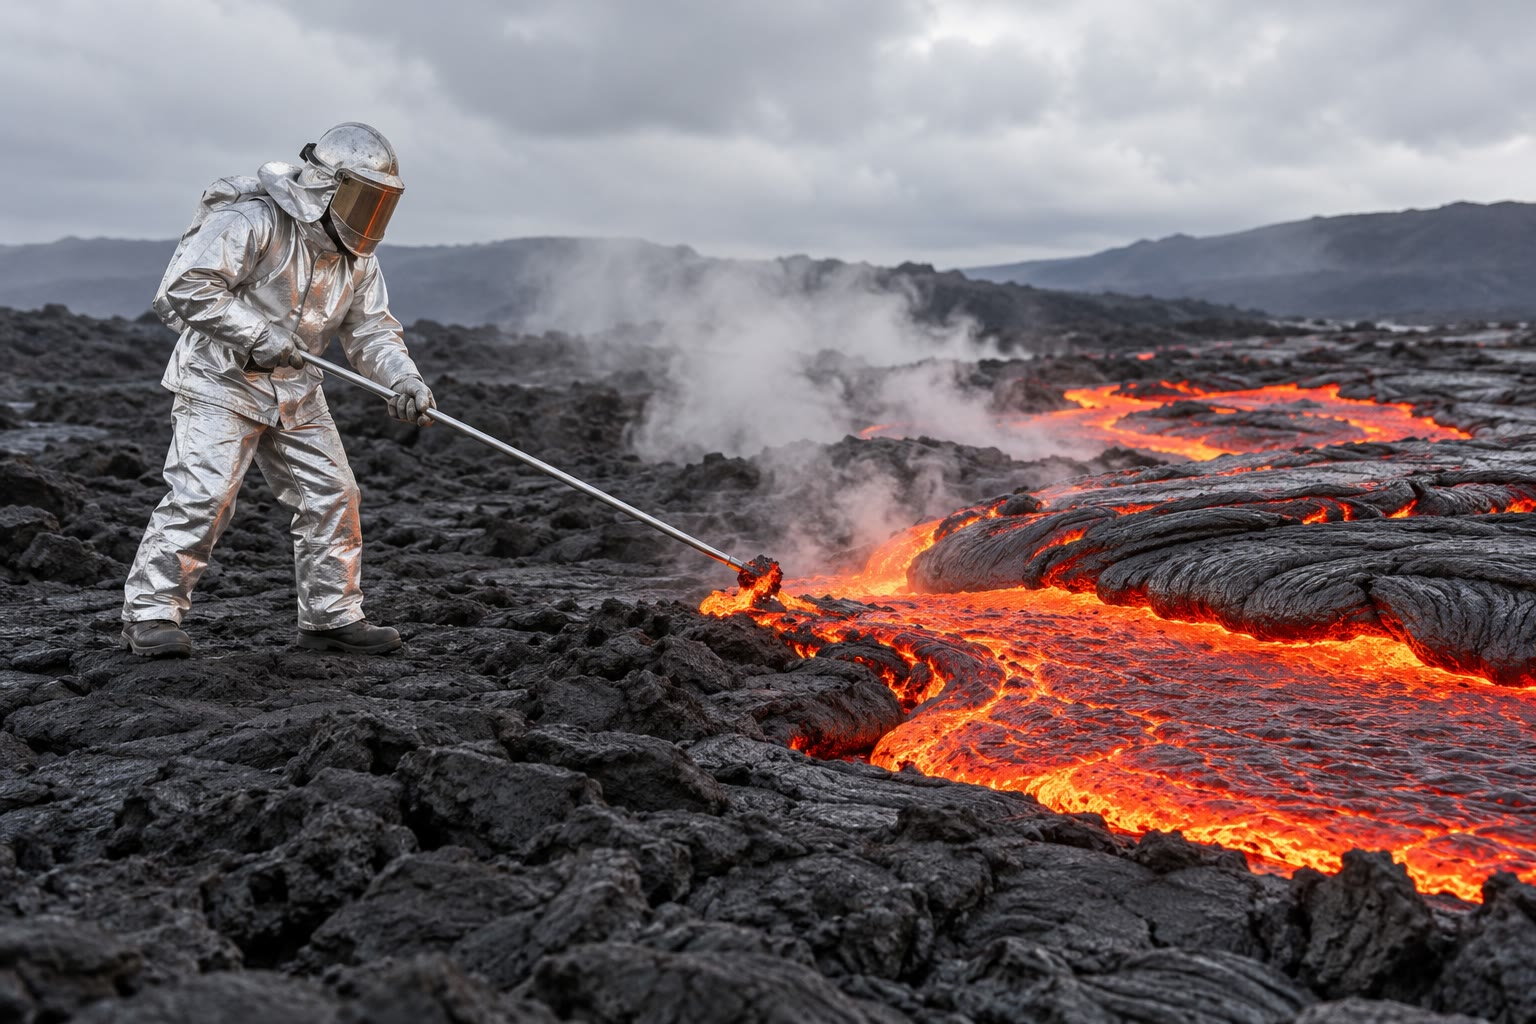
\includegraphics[width=0.6\linewidth]{images/book1/ai/g7-volcanologist.jpg}

{\small गर्मी लौटाने वाला सूट पहने एक \omterm{def:g4:volcanoes-earthquakes-first-look:volcano}{ज्वालामुखी} वैज्ञानिक इस्पात के एक लंबे
डंडे से \omterm{def:g4:volcanoes-earthquakes-first-look:eruption}{लावा} का नमूना लेता है (एक सामान्य दृश्य का AI चित्रण)। केवल
प्रशिक्षित वैज्ञानिक, इस तरह के उपकरणों के साथ, बहते \omterm{def:g4:volcanoes-earthquakes-first-look:eruption}{लावा} के पास जाते हैं;
बाकी सब वहीं से देखते हैं जहाँ अधिकारी अनुमति देते हैं।}
\label{fig:g7:volcanoes:volcanologist}
\end{omfigure}

\section{उद्गार के दो तरीके}

माउंट सेंट~हेलेंस ने खुद को उड़ा दिया। इसके उलट, हवाई के \omterm{def:g4:volcanoes-earthquakes-first-look:volcano}{ज्वालामुखी} आमतौर पर
\omterm{def:g4:volcanoes-earthquakes-first-look:eruption}{लावा} बहाते हैं जो उनकी ढलानों से नीचे बह जाता है। भूवैज्ञानिक \omterm{def:g4:volcanoes-earthquakes-first-look:eruption}{उद्गारों} को दो
प्रकारों में बाँटते हैं।

\begin{definition}[बहिःस्रावी और विस्फोटक उद्गार]\label{def:g7:volcanoes:eruption-types}
\emph{बहिःस्रावी उद्गार}\index{बहिःस्रावी उद्गार} में \omterm{def:g7:volcanoes:magma}{मैग्मा} शांति से \omterm{def:g4:volcanoes-earthquakes-first-look:eruption}{लावा}
बनकर बाहर आता है, जो \omterm{def:g7:volcanoes:vent}{निकास-छिद्र} से दूर बह जाता है, कभी-कभी किलोमीटरों तक, या
चमकती बूँदों के फव्वारों में ऊपर उछलता है। \emph{विस्फोटक
उद्गार}\index{विस्फोटक उद्गार} में \omterm{def:g7:volcanoes:magma}{मैग्मा} अपनी ही गैस से टुकड़े-टुकड़े हो जाता
है: राख, गैस और \omterm{def:g3:stones-pebbles-sand:rock}{चट्टान} के ढेलों का एक स्तंभ आकाश में बहुत ऊँचा फेंका जाता
है।
\end{definition}

\begin{omfigure}
\begin{minipage}[t]{0.49\linewidth}\centering
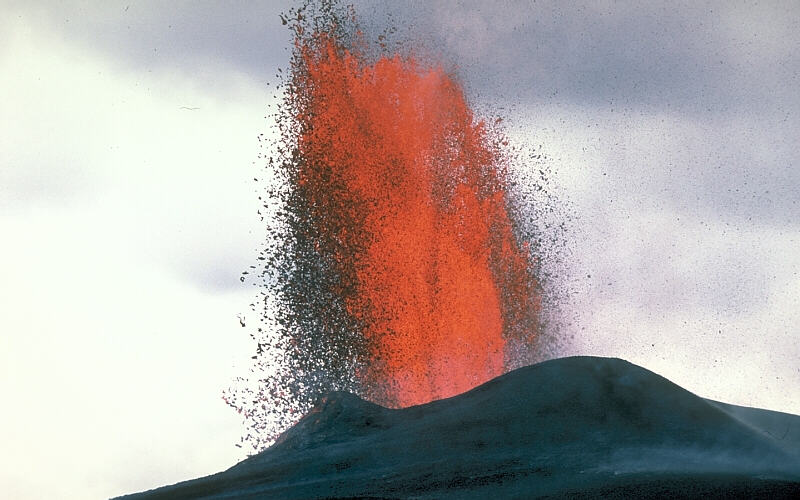
\includegraphics[height=4.5cm]{images/book1/g7-lava-fountain.jpg}

{\small बहिःस्रावी: किलाउआ, हवाई में \omterm{def:g4:volcanoes-earthquakes-first-look:eruption}{लावा} का एक फव्वारा, 1983।
फ़ोटो: ग्रिग्स, USGS।}
\end{minipage}\hfill
\begin{minipage}[t]{0.49\linewidth}\centering
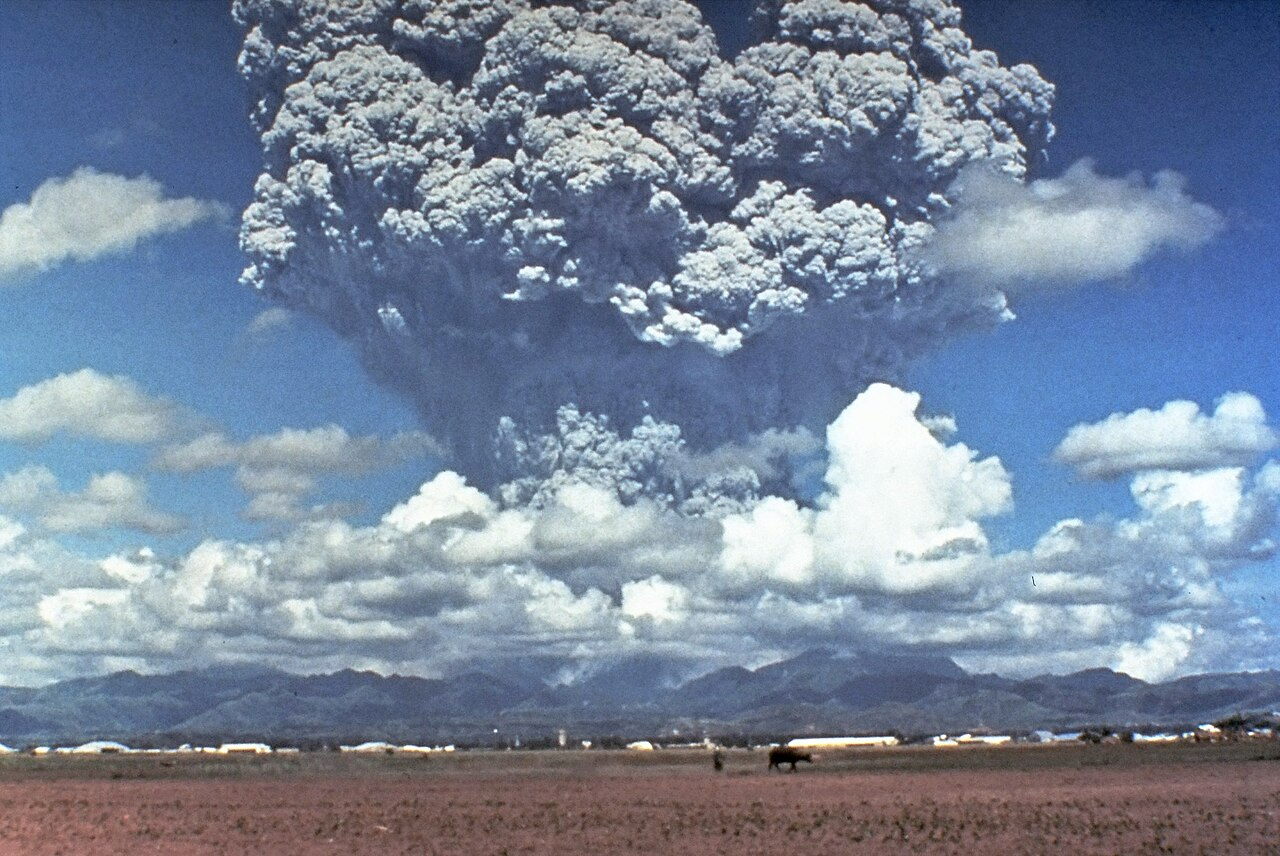
\includegraphics[height=4.5cm]{images/book1/g7-pinatubo.jpg}

{\small विस्फोटक: माउंट पिनातूबो, फ़िलिपींस, का \omterm{def:g4:volcanoes-earthquakes-first-look:eruption}{उद्गार} स्तंभ,
12~जून 1991। फ़ोटो: डेव हारलो, USGS।}
\end{minipage}\par\medskip


{\small दोनों तस्वीरें सार्वजनिक डोमेन में हैं (विकिमीडिया
कॉमन्स के ज़रिए)।}
% ledger: commons:lava-fountain, commons:pinatubo
\label{fig:g7:volcanoes:two-photos}
\end{omfigure}

फ़र्क़ किससे पड़ता है? दो चीज़ों से: \omterm{def:g7:volcanoes:magma}{मैग्मा} कितना पतला है, और उसमें कितनी गैस
है।

\textbf{पतला या चिपचिपा।} कुछ \omterm{def:g7:volcanoes:magma}{मैग्मा} पतला होता है, लगभग गुनगुने शहद जैसा: यह उस
\omterm{def:g7:volcanoes:magma}{मैग्मा} की बात है जो ठंडा होकर गहरे रंग का बेसाल्ट बनता है, जैसे हवाई में। दूसरा
\omterm{def:g7:volcanoes:magma}{मैग्मा} गाढ़ा और चिपचिपा होता है, ठंडे शहद या टूथपेस्ट जैसा। पतले \omterm{def:g7:volcanoes:magma}{मैग्मा} में
गैस के बुलबुले आसानी से ऊपर उठते हैं और सतह पर, थोड़े-थोड़े करके, निकल जाते हैं।
चिपचिपे \omterm{def:g7:volcanoes:magma}{मैग्मा} में बुलबुले फँस जाते हैं।

\textbf{कम या ज़्यादा गैस।} सोडा वाटर की एक बोतल में पानी में बहुत-सी गैस घुली
होती है, जिसे बंद बोतल के अंदर का दाब वहाँ रोके रखता है; वह दिखाई नहीं देती।
बोतल खोलो तो दाब गिर जाता है: हर जगह बुलबुले दिखने लगते हैं, और अगर बोतल
हिलाई गई हो, तो झाग फूटकर बाहर निकलता है। ज़मीन के बहुत नीचे \omterm{def:g7:volcanoes:magma}{मैग्मा} में भी ऊँचे
दाब पर गैस घुली होती है। जैसे-जैसे वह ऊपर उठता है, दाब गिरता है और गैस घोल से
बाहर निकलकर बुलबुले बन जाती है।
% ledger: usgs:volcanic-gases

दोनों को साथ रखो। कम गैस वाला पतला \omterm{def:g7:volcanoes:magma}{मैग्मा} अपने बुलबुलों को जाने देता है और
बहते \omterm{def:g4:volcanoes-earthquakes-first-look:eruption}{लावा} के रूप में बाहर आता है: \omterm{def:g4:volcanoes-earthquakes-first-look:eruption}{उद्गार} बहिःस्रावी होता है। गैस से भरा
चिपचिपा \omterm{def:g7:volcanoes:magma}{मैग्मा} अपने बुलबुलों को तब तक रोके रखता है जब तक वे इतने नहीं फूल जाते
कि \omterm{def:g7:volcanoes:magma}{मैग्मा} को चिथड़ों में फाड़ दें: \omterm{def:g4:volcanoes-earthquakes-first-look:eruption}{उद्गार} विस्फोटक होता है। झागदार \omterm{def:g7:volcanoes:magma}{मैग्मा} के
चिथड़े हवा में जमकर राख और झाँवा बन जाते हैं, एक \omterm{def:g3:stones-pebbles-sand:rock}{चट्टान} जो बुलबुलों से इतनी
भरी होती है कि पानी पर तैर सकती है।

\begin{example}[पिनातूबो, 1991: बेदम सोडा और हिलाया हुआ सोडा]\label{ex:g7:volcanoes:pinatubo}
% ledger: usgs:pinatubo-1991
जून~1991 में पहला \omterm{def:g7:volcanoes:magma}{मैग्मा} फ़िलिपींस में माउंट पिनातूबो की सतह तक पहुँचा। ऊपर
आते हुए वह अपनी ज़्यादातर गैस खो चुका था, निगरानी कर रहे वैज्ञानिकों के शब्दों
में ``बेदम हो चुकी सोडा की बोतल की तरह''। वह धीरे-धीरे रिसकर बाहर आया और
\omterm{def:g7:volcanoes:vent}{निकास-छिद्र} के ऊपर एक टीले के रूप में जमा हो गया: कोई विस्फोट नहीं। फिर
12~जून को अब भी गैस से भरा \omterm{def:g7:volcanoes:magma}{मैग्मा} सतह तक पहुँचा और फट पड़ा --- ऊपर वाली
तस्वीर का स्तंभ। 15~जून को और भी ज़्यादा गैस वाला \omterm{def:g7:volcanoes:magma}{मैग्मा} आया, और \omterm{def:g4:volcanoes-earthquakes-first-look:volcano}{ज्वालामुखी} में
बीसवीं सदी के सबसे बड़े \omterm{def:g4:volcanoes-earthquakes-first-look:eruption}{उद्गारों} में से एक हुआ: उसने पाँच घन किलोमीटर से ज़्यादा
\omterm{def:g3:stones-pebbles-sand:rock}{चट्टान} और राख बाहर फेंकी, उसका राख का \omterm{def:g4:clouds-rain-snow:cloud}{बादल} \qty{35}{km} ऊँचा उठा, और पहाड़ की
चोटी धँसकर \qty{2.5}{km} चौड़ा एक गड्ढा बन गई। वही \omterm{def:g4:volcanoes-earthquakes-first-look:volcano}{ज्वालामुखी}, वही हफ़्ता: फ़र्क़
गैस ने डाला।
\end{example}

\omterm{def:g4:volcanoes-earthquakes-first-look:volcano}{ज्वालामुखी} का आकार उसके \omterm{def:g4:volcanoes-earthquakes-first-look:eruption}{उद्गारों} की याद सँजोकर रखता है। पतला \omterm{def:g4:volcanoes-earthquakes-first-look:eruption}{लावा} सख़्त होने से
पहले दूर तक बहता है, इसलिए परत-दर-परत वह हल्की ढलानों वाला एक चौड़ा पहाड़
बनाता है, जिसका आकार ज़मीन पर रखी किसी योद्धा की ढाल जैसा होता है: एक
\emph{शील्ड \omterm{def:g4:volcanoes-earthquakes-first-look:volcano}{ज्वालामुखी}}। हवाई में मौना लोआ ऐसा ही है। चिपचिपा \omterm{def:g4:volcanoes-earthquakes-first-look:eruption}{लावा} और राख
\omterm{def:g7:volcanoes:vent}{निकास-छिद्र} के पास ही जमा हो जाते हैं, और \omterm{def:g4:volcanoes-earthquakes-first-look:eruption}{लावा} और राख की परतों से बना एक खड़ा
शंकु बनाते हैं: एक \emph{स्तरित \omterm{def:g4:volcanoes-earthquakes-first-look:volcano}{ज्वालामुखी}} (\emph{स्तर} यानी परतें)। माउंट
सेंट~हेलेंस और पिनातूबो ऐसे दो \omterm{def:g4:volcanoes-earthquakes-first-look:volcano}{ज्वालामुखी} हैं।

\begin{omfigure}
\begin{tikzpicture}[font=\small, x=1cm, y=1cm]
  % --- left: effusive, a shield
  \begin{scope}
    \fill[brown!25] (-3.3,-1.2) rectangle (3.3,0);
    \fill[black!50] (-3.3,0) .. controls (-2.0,0.45) and (-1.0,1.0) .. (-0.35,1.25)
      -- (0.35,1.25) .. controls (1.0,1.0) and (2.0,0.45) .. (3.3,0) -- cycle;
    \fill[orange!85!red] (-0.12,-1.2) rectangle (0.12,1.25);
    % fountain
    \foreach \a in {-25,-12,0,12,25}
      \draw[orange!90!red, line width=0.9pt] (0,1.25) .. controls ({0.4*sin(\a)},2.2) .. ({1.0*sin(\a)},1.6);
    % lava flows far down the gentle slopes
    \draw[orange!95!red, line width=2.2pt, line cap=round] (0.3,1.22) .. controls (1.2,0.95) and (2.1,0.45) .. (3.1,0.08);
    \draw[orange!95!red, line width=2.2pt, line cap=round] (-0.3,1.22) .. controls (-1.3,0.95) and (-2.2,0.45) .. (-3.0,0.1);
    \node[font=\small\bfseries] at (0,4.3) {बहिःस्रावी};
    \node[align=center, font=\footnotesize] at (0,-1.75) {पतला मैग्मा, कम गैस:\\लावा दूर तक बहता है; एक चौड़ी ढाल};
    \node[anchor=west, font=\footnotesize] at (1.2,1.9) {लावा का फव्वारा};
    \draw[black!60] (1.15,1.9) -- (0.6,1.75);
    \node[anchor=west, font=\footnotesize, align=left] at (1.9,1.2) {लावा के लंबे\\प्रवाह};
    \draw[black!60] (1.85,1.05) -- (1.5,0.82);
  \end{scope}
  % --- right: explosive, a steep cone
  \begin{scope}[xshift=7.4cm]
    \fill[brown!25] (-3.3,-1.2) rectangle (3.3,0);
    \fill[black!45] (-2.3,0) -- (-0.4,2.2) -- (0.4,2.2) -- (2.3,0) -- cycle;
    \fill[orange!85!red] (-0.12,-1.2) rectangle (0.12,2.2);
    \foreach \x/\y/\r in {0/2.6/0.35, -0.3/3.05/0.4, 0.3/3.1/0.38, 0/3.5/0.45, -0.45/3.55/0.32, 0.45/3.6/0.32}
      \fill[black!28] (\x,\y) circle (\r);
    % pyroclastic flow down the flank
    \fill[black!30] (0.45,2.1) .. controls (1.0,1.5) and (1.6,0.7) .. (2.9,0.05)
      -- (2.2,0.05) .. controls (1.4,0.45) and (0.9,1.2) .. (0.35,1.95) -- cycle;
    \node[font=\small\bfseries] at (0,4.3) {विस्फोटक};
    \node[align=center, font=\footnotesize] at (0,-1.75) {चिपचिपा मैग्मा, ज़्यादा गैस:\\राख का स्तंभ; एक खड़ा शंकु};
    \node[anchor=west, font=\footnotesize] at (0.9,3.4) {राख का स्तंभ};
    \draw[black!60] (0.85,3.4) -- (0.7,3.4);
    \node[anchor=west, font=\footnotesize, align=left] at (1.8,1.35) {पायरोक्लास्टिक\\प्रवाह};
    \draw[black!60] (1.75,1.35) -- (1.3,1.0);
  \end{scope}
\end{tikzpicture}

{\small \omterm{def:g4:volcanoes-earthquakes-first-look:eruption}{उद्गार} के दो प्रकार और वे \omterm{def:g4:volcanoes-earthquakes-first-look:volcano}{ज्वालामुखी} जो वे बनाते हैं (चित्र, पैमाने पर
नहीं)।}
\label{fig:g7:volcanoes:two-kinds}
\end{omfigure}

\begin{method}[बहिःस्रावी या विस्फोटक? चार सुराग]\label{met:g7:volcanoes:clues}
किसी वर्णन या तस्वीर से यह बताने के लिए कि किसी \omterm{def:g4:volcanoes-earthquakes-first-look:volcano}{ज्वालामुखी} का \omterm{def:g4:volcanoes-earthquakes-first-look:eruption}{उद्गार} किस तरह का
है, ये सुराग ढूँढो।
\begin{enumerate}
  \item \emph{क्या बाहर आता है?} बहता या फव्वारों में उछलता \omterm{def:g4:volcanoes-earthquakes-first-look:eruption}{लावा}:
        बहिःस्रावी। राख का स्तंभ, बाहर फेंके गए \omterm{def:g3:stones-pebbles-sand:rock}{चट्टान} के ढेले: विस्फोटक।
  \item \emph{\omterm{def:g4:volcanoes-earthquakes-first-look:volcano}{ज्वालामुखी} का आकार।} हल्की ढलानों वाला चौड़ा पहाड़: ज़्यादातर
        \omterm{def:g7:volcanoes:eruption-types}{बहिःस्रावी उद्गार}। खड़ा शंकु: अक्सर विस्फोटक।
  \item \emph{\omterm{def:g7:volcanoes:magma}{मैग्मा}।} पतला, कम गैस: बहिःस्रावी। चिपचिपा, ज़्यादा गैस:
        विस्फोटक।
  \item \emph{पीछे छूटी \omterm{def:g3:stones-pebbles-sand:rock}{चट्टानें}।} गहरे रंग के, ठोस \omterm{def:g4:volcanoes-earthquakes-first-look:eruption}{लावा} प्रवाह: बहिःस्रावी।
        राख और झाँवे की परतें: विस्फोटक।
\end{enumerate}
\end{method}

\begin{example}[सुरागों का उपयोग]\label{ex:g7:volcanoes:clues}
एक यात्री एक \omterm{def:g4:volcanoes-earthquakes-first-look:volcano}{ज्वालामुखी} का वर्णन करता है: ``एक विशाल, हल्का गोलाई लिए पहाड़,
उसकी ढलानों पर हर जगह काले \omterm{def:g4:volcanoes-earthquakes-first-look:eruption}{लावा} प्रवाह, उनमें से कुछ केवल कुछ साल पुराने''।
सुराग~2 (हल्की ढलानें) और सुराग~4 (गहरे रंग के \omterm{def:g4:volcanoes-earthquakes-first-look:eruption}{लावा} प्रवाह) दोनों \omterm{def:g7:volcanoes:eruption-types}{बहिःस्रावी
उद्गारों} की ओर इशारा करते हैं: यह मौना लोआ जैसा एक शील्ड \omterm{def:g4:volcanoes-earthquakes-first-look:volcano}{ज्वालामुखी} है।
\end{example}

\begin{inthelab}[बोतल में ज्वालामुखी (कक्षा में, अध्यापक के साथ)]
अध्यापक सोडा वाटर की दो बंद बोतलें लेते हैं। एक को खड़ा छोड़ दिया गया है; दूसरी
को धीरे से हिलाया गया है। दोनों को बाहर, एक टब के ऊपर, सबसे दूर की ओर मुँह करके
खोला जाता है। शांत बोतल फुसफुसाती है और कुछ बुलबुले ऊपर उठने देती है; हिलाई
हुई बोतल झाग बनकर फूट पड़ती है जो बाहर उछलता है। कौन-सी बोतल हवाई के \omterm{def:g7:volcanoes:magma}{मैग्मा}
जैसी है, और कौन-सी पिनातूबो के \omterm{def:g7:volcanoes:magma}{मैग्मा} जैसी? फिर पानी के एक कटोरे में झाँवे का
एक टुकड़ा और एक \omterm{def:g3:stones-pebbles-sand:pebble}{कंकड़} डालो: झाँवा तैरता है। उसे आवर्धक लेंस से देखो: वह छेदों
से भरा है, जो गैस के वे बुलबुले हैं जो \omterm{def:g7:volcanoes:magma}{मैग्मा} के फटते समय \omterm{def:g3:stones-pebbles-sand:rock}{चट्टान} में जम
गए।
\end{inthelab}

\section{ज्वालामुखी से क्या बाहर आता है}

\omterm{def:g4:volcanoes-earthquakes-first-look:eruption}{उद्गार} \omterm{def:g4:volcanoes-earthquakes-first-look:eruption}{लावा} से कहीं ज़्यादा बाहर फेंकता है: गैसें, राख, \omterm{def:g3:stones-pebbles-sand:rock}{चट्टान} के ढेले और,
सबसे बुरे मामलों में, गरम राख के हिमस्खलन।

सबसे ज़्यादा मात्रा वाली गैस, बहुत बड़े अंतर से, जलवाष्प है। बड़े \omterm{def:g4:volcanoes-earthquakes-first-look:eruption}{उद्गार} थोड़े
समय में भारी मात्रा में गैस छोड़ते हैं: माना जाता है कि 1991 के एक ही दिन में
पिनातूबो ने 250~मिलियन टन से ज़्यादा गैस ऊपरी वायुमंडल में
भेजी।
% ledger: usgs:volcanic-gases

\begin{definition}[पायरोक्लास्टिक प्रवाह]\label{def:g7:volcanoes:pyroclastic-flow}
\emph{पायरोक्लास्टिक प्रवाह}\index{पायरोक्लास्टिक प्रवाह} गरम गैस, राख और
\omterm{def:g3:stones-pebbles-sand:rock}{चट्टान} के टुकड़ों का, धूल के कणों से लेकर बड़े शिलाखंडों तक, एक तेज़ हिमस्खलन है,
जो \omterm{def:g7:volcanoes:eruption-types}{विस्फोटक उद्गार} के दौरान \omterm{def:g4:volcanoes-earthquakes-first-look:volcano}{ज्वालामुखी} की ढलानों से नीचे दौड़ता है।
(यूनानी में \emph{पायरो} का अर्थ आग है और \emph{क्लास्टिक} का अर्थ टूटे टुकड़ों से बना।)
\end{definition}

\omterm{def:g7:volcanoes:pyroclastic-flow}{पायरोक्लास्टिक प्रवाह} आमतौर पर \qty{80}{km/h} से ज़्यादा तेज़ चलते हैं, और उनके
अंदर की \omterm{def:g3:stones-pebbles-sand:rock}{चट्टानें} और गैस आमतौर पर 200 से \qty{700}{\degreeCelsius} के बीच होती
हैं। वे आमतौर पर पानी की तरह \omterm{def:g1:landscapes-around-us:landform}{घाटियों} के साथ चलते हैं, और अपने रास्ते में आने वाली
लगभग हर चीज़ को गिरा देते हैं, जला देते हैं या दबा देते हैं। 18~मई 1980 को माउंट
सेंट~हेलेंस के \omterm{def:g7:volcanoes:pyroclastic-flow}{पायरोक्लास्टिक प्रवाह} 80 से \qty{130}{km/h} की चाल से, कम से कम
\qty{700}{\degreeCelsius} तापमान पर, दौड़े और \omterm{def:g7:volcanoes:vent}{क्रेटर} से \qty{8}{km} तक पहुँचे।
% ledger: usgs:pyroclastic-flows, usgs:msh-flows, usgs:msh-reach

तालिका \omterm{def:g4:volcanoes-earthquakes-first-look:volcano}{ज्वालामुखी} के उत्पादों का सार देती है।

\begin{center}
\small
\begin{tabular}{|p{0.2\linewidth}|p{0.4\linewidth}|p{0.3\linewidth}|}
\hline
\textbf{उत्पाद} & \textbf{यह क्या है} & \textbf{ख़तरा} \\
\hline
\omterm{def:g4:volcanoes-earthquakes-first-look:eruption}{लावा} प्रवाह & ज़मीन पर बहती, फिर सख़्त होती पिघली \omterm{def:g3:stones-pebbles-sand:rock}{चट्टान} & जिससे मिलता है उसे जलाता और दबा देता है, पर आमतौर पर इतना धीमा होता है कि लोग रास्ते से हट सकें \\
\hline
राख & \omterm{def:g3:stones-pebbles-sand:rock}{चट्टान} और काँच के नन्हे टुकड़े, हवा में उड़ाए गए & बहुत दूर गिरती है; उसके भार से छतें गिर जाती हैं; वह विमानों को नुकसान पहुँचाती है \\
\hline
\omterm{def:g4:volcanoes-earthquakes-first-look:volcano}{ज्वालामुखी} बम & बाहर फेंके गए \omterm{def:g4:volcanoes-earthquakes-first-look:eruption}{लावा} के ढेले, जो उड़ते हुए सख़्त हो जाते हैं & \omterm{def:g7:volcanoes:vent}{निकास-छिद्र} के पास, जिससे टकराते हैं उसे कुचल देते हैं \\
\hline
गैसें & ज़्यादातर जलवाष्प, फिर कार्बन डाइऑक्साइड और सल्फ़र डाइऑक्साइड & कुछ ज़हरीली हैं; कार्बन डाइऑक्साइड गड्ढों में जमा हो जाती है \\
\hline
\omterm{def:g7:volcanoes:pyroclastic-flow}{पायरोक्लास्टिक प्रवाह} & गरम राख, \omterm{def:g3:stones-pebbles-sand:rock}{चट्टान} और गैस का हिमस्खलन & सबसे जानलेवा: बच निकलने के लिए बहुत तेज़ और बहुत गरम \\
\hline
कीचड़ प्रवाह & \omterm{def:g4:clouds-rain-snow:precipitation}{बारिश} या पिघली बर्फ़ के पानी में मिली राख और \omterm{def:g3:stones-pebbles-sand:rock}{चट्टान} & \omterm{def:g1:landscapes-around-us:landform}{घाटियों} में नीचे दौड़ता है, कभी-कभी \omterm{def:g4:volcanoes-earthquakes-first-look:volcano}{ज्वालामुखी} से बहुत दूर तक \\
\hline
\end{tabular}
\end{center}
% ledger: usgs:lava-flows, usgs:volcanic-gases, usgs:pyroclastic-flows, usgs:pinatubo-1991, usgs:msh-flows

\begin{method}[कितना समय लगता है?]\label{met:g7:volcanoes:time}
यह जानने के लिए कि किसी ज्ञात चाल से चलने वाली कोई चीज़ एक दूरी तय करने में
कितना समय लेती है, दूरी को चाल से भाग दो:
\[
\text{समय} = \frac{\text{दूरी}}{\text{चाल}}.
\]
दूरी किलोमीटर में और चाल किलोमीटर प्रति घंटा में हो, तो समय घंटों में आता है;
मिनट पाने के लिए 60 से गुणा करो।
\end{method}

\begin{example}[पायरोक्लास्टिक प्रवाह से दौड़]\label{ex:g7:volcanoes:race}
\qty{120}{km/h} की चाल से चलता एक \omterm{def:g7:volcanoes:pyroclastic-flow}{पायरोक्लास्टिक प्रवाह} \omterm{def:g1:landscapes-around-us:landform}{घाटी} में नीचे
\qty{6}{km} दूर एक गाँव की ओर बढ़ता है। उसे $6 \div 120 = 0.05$~घंटा लगता है,
यानी $0.05 \times 60 = 3$~मिनट। तीन मिनट: कोई भी समय रहते दौड़कर, या गाड़ी
चलाकर भी, \omterm{def:g1:landscapes-around-us:landform}{घाटी} से बाहर नहीं निकल सकता। लोग तभी सुरक्षित हैं जब वे \omterm{def:g4:volcanoes-earthquakes-first-look:eruption}{उद्गार} से
\emph{पहले} निकल चुके हों।
\end{example}

\begin{remark}[कीचड़ प्रवाह: बाद में आने वाला ख़तरा]\label{rem:g7:volcanoes:mudflows}
% ledger: usgs:msh-flows, usgs:pinatubo-lahars
\omterm{def:g4:volcanoes-earthquakes-first-look:eruption}{उद्गार} ढलानों को ढीली राख से ढका छोड़ जाता है। जब उस पर \omterm{def:g4:clouds-rain-snow:precipitation}{बारिश} गिरती है, या जब
गर्मी चोटी की बर्फ़ को पिघला देती है, तो राख कीचड़ प्रवाहों में बदल जाती है जो
\omterm{def:g1:landscapes-around-us:landform}{घाटियों} में नीचे दौड़ते हैं। 18~मई 1980 को माउंट सेंट~हेलेंस के कीचड़ प्रवाहों ने
27~पुलों और लगभग 200~घरों को नुकसान पहुँचाया। पिनातूबो के आसपास, बाद के वर्षों
की भारी \omterm{def:g4:clouds-rain-snow:precipitation}{बारिशों} ने राख को विशाल कीचड़ प्रवाहों में बदल दिया जिन्होंने पूरे के
पूरे गाँव दबा दिए: उन्होंने ख़ुद \omterm{def:g4:volcanoes-earthquakes-first-look:eruption}{उद्गार} से ज़्यादा नुकसान
किया।
\end{remark}


\section{ज्वालामुखी कहाँ हैं?}

वॉशिंगटन का स्मिथसोनियन संस्थान उन सभी \omterm{def:g4:volcanoes-earthquakes-first-look:volcano}{ज्वालामुखियों} की एक सूची रखता है जिनके
बारे में पता है कि वे पिछले 12\,000 वर्षों में फटे हैं: ज़मीन पर और \omterm{def:g2:water-on-earth:ocean}{समुद्र} के
नीचे, कुल 1\,214। हर एक के लिए सूची बताती है कि वह \omterm{def:g7:plate-tectonics:plate}{प्लेटों} के सापेक्ष कहाँ
स्थित है। नीचे का \omterm{def:g2:drawing-to-map:map}{मानचित्र} उन्हें इसी के अनुसार रंगता है।
% ledger: data:gvp (counts computed in figdata/grade-7/volcano_settings.py)

\begin{omfigure}
\begin{tikzpicture}
\begin{axis}[ommap, width=\linewidth, xtick={-180,-90,...,180}, ytick={-60,0,60},
  legend style={at={(0.02,0.04)}, anchor=south west, font=\scriptsize,
  fill=white, fill opacity=0.85, text opacity=1, draw=black!40}, legend cell align=left]
\addplot[fill=omLithAlluv, draw=black!45, line width=0.2pt, forget plot] table {figdata/out/shared-geo-land.dat};
\addplot[omRidge!60, line width=0.5pt, forget plot] table {figdata/out/shared-geo-school-ridge.dat};
\addplot[omTrench!60, line width=0.5pt, forget plot] table {figdata/out/shared-geo-school-subduction.dat};
\addplot[only marks, mark=triangle*, mark size=1.3pt, omTrench, forget plot] table {figdata/out/grade-7-volcano_settings-map-sub.dat};
\addplot[only marks, mark=triangle*, mark size=1.3pt, omRidge, forget plot] table {figdata/out/grade-7-volcano_settings-map-rift.dat};
\addplot[only marks, mark=*, mark size=1.4pt, orange!90!black, forget plot] table {figdata/out/grade-7-volcano_settings-map-intra.dat};
\addlegendimage{only marks, mark=triangle*, mark size=1.6pt, omTrench}
\addlegendentry{जहाँ एक प्लेट दूसरी के नीचे धँसती है}
\addlegendimage{only marks, mark=triangle*, mark size=1.6pt, omRidge}
\addlegendentry{जहाँ प्लेटें एक-दूसरे से दूर जाती हैं}
\addlegendimage{only marks, mark=*, mark size=1.6pt, orange!90!black}
\addlegendentry{किसी प्लेट के अंदर}
\end{axis}
\end{tikzpicture}

{\small पिछले 12\,000 वर्षों में सक्रिय \omterm{def:g4:volcanoes-earthquakes-first-look:volcano}{ज्वालामुखी}, उनकी स्थिति के अनुसार रंगे
हुए। हल्की रेखाएँ: वे \omterm{def:g7:plate-tectonics:plate-boundary}{प्लेट सीमाएँ} जहाँ \omterm{def:g7:plate-tectonics:plate}{प्लेटें} एक-दूसरे से दूर जाती हैं (लाल)
और जहाँ एक \omterm{def:g7:plate-tectonics:plate}{प्लेट} दूसरी के नीचे धँसती है (नीली)। आँकड़े: स्मिथसोनियन ग्लोबल
वोल्कैनिज़्म प्रोग्राम; सीमाएँ बर्ड (2003) के अनुसार; तटरेखाएँ नैचुरल अर्थ
से।}
% ledger: data:gvp, data:pb2002, data:ne-land
\label{fig:g7:volcanoes:map}
\end{omfigure}

\begin{omfigure}
\begin{tikzpicture}
  \begin{axis}[xbar, width=0.72\linewidth, height=3.6cm, bar width=8pt,
      xmin=0, xmax=1000, ymin=-0.6, ymax=3.6, y dir=reverse,
      ytick={0,...,3}, yticklabels={जहाँ एक प्लेट दूसरी के नीचे धँसती है, जहाँ प्लेटें दूर जाती हैं, किसी प्लेट के अंदर, ज्ञात नहीं},
      xlabel={ज्वालामुखियों की संख्या},
      axis x line=bottom, axis y line=left, axis line style={-},
      tick label style={font=\scriptsize}, label style={font=\small},
      nodes near coords, nodes near coords style={font=\scriptsize, anchor=west},
      point meta=explicit symbolic, enlarge y limits=false, clip=false]
    \addplot[fill=black!30, draw=black!60] table[x=n, y=idx, meta=n] {figdata/out/grade-7-volcano_settings.dat};
  \end{axis}
\end{tikzpicture}

{\small 1\,214 \omterm{def:g4:volcanoes-earthquakes-first-look:volcano}{ज्वालामुखियों} में से कितने किस स्थिति में हैं।}
% ledger: data:gvp (figdata/grade-7/volcano_settings.py, main table)
\label{fig:g7:volcanoes:counts}
\end{omfigure}

\begin{proposition}[ज़्यादातर ज्वालामुखी प्लेट सीमाओं पर हैं]\label{prop:g7:volcanoes:where}
% ledger: data:gvp (counts computed in figdata/grade-7/volcano_settings.py)
पिछले 12\,000 वर्षों में सक्रिय 1\,214 \omterm{def:g4:volcanoes-earthquakes-first-look:volcano}{ज्वालामुखियों} में से 838 (69~\%) वहाँ हैं
जहाँ एक \omterm{def:g7:plate-tectonics:plate}{प्लेट} दूसरी के नीचे धँसती है और 221 (18~\%) वहाँ जहाँ \omterm{def:g7:plate-tectonics:plate}{प्लेटें} एक-दूसरे
से दूर जाती हैं; 149 (12~\%) किसी \omterm{def:g7:plate-tectonics:plate}{प्लेट} के अंदर, उसके किनारों से दूर, हैं। बाकी
6 (0.5~\%) की स्थिति ज्ञात नहीं है।
\end{proposition}

\textbf{जहाँ \omterm{def:g7:plate-tectonics:plate}{प्लेटें} एक-दूसरे से दूर जाती हैं।} महासागरीय कटकों के साथ-साथ, और
पूर्वी अफ़्रीका को फाड़ रही दरार \omterm{def:g1:landscapes-around-us:landform}{घाटी} जैसी दरार \omterm{def:g1:landscapes-around-us:landform}{घाटियों} में, \omterm{def:g7:plate-tectonics:plate}{प्लेटें} एक-दूसरे से
दूर खिंचती हैं। \omterm{def:g6:inside-the-earth:layers}{प्रावार} से \omterm{def:g7:volcanoes:magma}{मैग्मा} चौड़ी होती दरारों में ऊपर उठता है और उन्हें भर
देता है: नई \omterm{def:g6:inside-the-earth:layers}{भूपर्पटी} बनती है। ज़्यादातर कटक \omterm{def:g2:water-on-earth:ocean}{समुद्र} के नीचे हैं, पर आइसलैंड ठीक
मध्य-अटलांटिक कटक पर है: वहाँ ये \omterm{def:g4:volcanoes-earthquakes-first-look:volcano}{ज्वालामुखी} ज़मीन पर देखे जा सकते हैं। उनका
\omterm{def:g7:volcanoes:magma}{मैग्मा} ज़्यादातर पतला बेसाल्टी \omterm{def:g7:volcanoes:magma}{मैग्मा} है, और उनके \omterm{def:g4:volcanoes-earthquakes-first-look:eruption}{उद्गार} ज़्यादातर बहिःस्रावी
होते हैं।
% ledger: usgs:arc-magma, usgs:iceland, usgs:east-africa

\textbf{जहाँ एक \omterm{def:g7:plate-tectonics:plate}{प्लेट} दूसरी के नीचे धँसती है।} तीन में से दो से ज़्यादा
\omterm{def:g4:volcanoes-earthquakes-first-look:volcano}{ज्वालामुखी} यहीं हैं, उन रेखाओं के साथ जो प्रशांत \omterm{def:g2:water-on-earth:ocean}{महासागर} के किनारों के साथ चलती
हैं --- ``अग्नि-वलय'' --- और कुछ दूसरी जगहों पर। बहुत नीचे, धँसती \omterm{def:g7:plate-tectonics:plate}{प्लेट} के
साथ-साथ, कुछ \omterm{def:g3:stones-pebbles-sand:rock}{चट्टान} आंशिक रूप से पिघलती है; वैज्ञानिक अब भी इस पर चर्चा करते हैं
कि ठीक-ठीक कौन-सी \omterm{def:g3:stones-pebbles-sand:rock}{चट्टान} पिघलती है, धँसती \omterm{def:g7:plate-tectonics:plate}{प्लेट} या उसके ऊपर की \omterm{def:g7:plate-tectonics:plate}{प्लेट}, या दोनों।
वहाँ ऊपर उठने वाला \omterm{def:g7:volcanoes:magma}{मैग्मा} अक्सर चिपचिपा और गैस से भरा होता है: ये विस्फोटक
\omterm{def:g4:volcanoes-earthquakes-first-look:volcano}{ज्वालामुखी} हैं, जैसे माउंट सेंट~हेलेंस और पिनातूबो। आँकड़े यही दिखाते हैं: सूची के
660 खड़े शंकुओं (स्तरित \omterm{def:g4:volcanoes-earthquakes-first-look:volcano}{ज्वालामुखियों}) में से 564 --- यानी 85~\% --- वहाँ हैं
जहाँ एक \omterm{def:g7:plate-tectonics:plate}{प्लेट} दूसरी के नीचे धँसती है।
% ledger: usgs:arc-magma, data:gvp (figdata/grade-7/volcano_settings.py, part strato)

\textbf{किसी \omterm{def:g7:plate-tectonics:plate}{प्लेट} के अंदर।} कुछ \omterm{def:g4:volcanoes-earthquakes-first-look:volcano}{ज्वालामुखी} किसी भी सीमा से दूर हैं। सबसे
प्रसिद्ध हवाई के \omterm{def:g4:volcanoes-earthquakes-first-look:volcano}{ज्वालामुखी} हैं, प्रशांत \omterm{def:g2:water-on-earth:ocean}{महासागर} के बीच में, किसी \omterm{def:g7:plate-tectonics:plate}{प्लेट} के सबसे
पास वाले किनारे से \qty{3200}{km} से भी ज़्यादा दूर।
% ledger: usgs:hawaii-hotspot

\begin{definition}[तप्त स्थल]\label{def:g7:volcanoes:hotspot}
\emph{तप्त स्थल}\index{तप्त स्थल} \omterm{def:g6:inside-the-earth:layers}{प्रावार} में गहरी एक जगह है जो मिलियनों
वर्षों तक गरम रहती है और सतह पर \omterm{def:g4:volcanoes-earthquakes-first-look:volcano}{ज्वालामुखियों} को \omterm{def:g7:volcanoes:magma}{मैग्मा} देती रहती है, \omterm{def:g7:plate-tectonics:plate}{प्लेटों}
के किनारों से दूर भी।
\end{definition}

\omterm{def:g7:volcanoes:hotspot}{तप्त स्थल} अपनी जगह पर रहता है, जबकि उसके ऊपर की \omterm{def:g7:plate-tectonics:plate}{प्लेट} चलती है। \omterm{def:g7:volcanoes:hotspot}{तप्त स्थल} के ऊपर
एक \omterm{def:g4:volcanoes-earthquakes-first-look:volcano}{ज्वालामुखी} बढ़ता है; फिर चलती \omterm{def:g7:plate-tectonics:plate}{प्लेट} उसे दूर ले जाती है, और वह मर जाता है,
जबकि उसके पीछे \omterm{def:g7:volcanoes:hotspot}{तप्त स्थल} के ऊपर एक नया \omterm{def:g4:volcanoes-earthquakes-first-look:volcano}{ज्वालामुखी} बढ़ता है। समय के साथ \omterm{def:g7:plate-tectonics:plate}{प्लेट}
\omterm{def:g4:volcanoes-earthquakes-first-look:volcano}{ज्वालामुखियों} की एक पूरी कतार ढोती है, जिसमें सबसे पुराना \omterm{def:g7:volcanoes:hotspot}{तप्त स्थल} से सबसे दूर
होता है। हवाई में हम ठीक यही देखते हैं: बसे हुए द्वीपों के उत्तर-पश्चिमी सिरे
पर काउआई द्वीप की सबसे पुरानी \omterm{def:g3:stones-pebbles-sand:rock}{चट्टानें} लगभग 5.5~मिलियन वर्ष पुरानी हैं, और
\omterm{def:g4:clouds-rain-snow:precipitation}{बारिश} और लहरों ने उन्हें गहराई तक घिस दिया है; दक्षिण-पूर्वी सिरे पर बिग
आइलैंड पर सतह की सबसे पुरानी \omterm{def:g3:stones-pebbles-sand:rock}{चट्टानें} 0.7~मिलियन वर्ष से कम पुरानी हैं, और वहाँ
अब भी नया \omterm{def:g4:volcanoes-earthquakes-first-look:eruption}{लावा} निकलता है।
% ledger: usgs:hawaii-hotspot

\begin{history}[एक भूभौतिकविद और द्वीपों की एक कतार]
% ledger: usgs:hawaii-hotspot
धरती की सबसे बड़ी \omterm{def:g7:plate-tectonics:plate}{प्लेट} के बीच में \omterm{def:g4:volcanoes-earthquakes-first-look:volcano}{ज्वालामुखी} द्वीपों की एक श्रृंखला क्यों उठनी
चाहिए? 1963 में कनाडा के भूभौतिकविद तूज़ो विल्सन ने एक जवाब सुझाया। उन्होंने
कहा कि हवाई के द्वीप एक कतार में इसलिए हैं क्योंकि प्रशांत \omterm{def:g7:plate-tectonics:plate}{प्लेट} \omterm{def:g6:inside-the-earth:layers}{प्रावार} में
गर्मी के एक गहरे, स्थिर स्रोत के ऊपर से चलती है, जो अपने ऊपर की \omterm{def:g7:plate-tectonics:plate}{प्लेट} को आंशिक
रूप से पिघलाता है। अगर वे सही थे, तो द्वीप बिग आइलैंड के सक्रिय \omterm{def:g4:volcanoes-earthquakes-first-look:volcano}{ज्वालामुखियों} से
जितने दूर हों, उतने ही पुराने और घिसे हुए होने चाहिए। उनकी \omterm{def:g3:stones-pebbles-sand:rock}{चट्टानों} की उम्रें ठीक यही दिखाती हैं। एक ही विचार ने कतार और उम्रों का क्रम, दोनों समझा दिए।
(विल्सन वही वैज्ञानिक भी हैं जिन्होंने \omterm{def:g7:plate-tectonics:plate-boundary}{रूपांतर सीमाओं} की खोज की, जहाँ \omterm{def:g7:plate-tectonics:plate}{प्लेटें}
एक-दूसरे के पास से सरकती हैं।)
\end{history}

\begin{omfigure}
\begin{tikzpicture}[font=\small, x=1cm, y=1cm]
  % sea, plate and mantle
  \fill[omSea!45] (-6.2,0) rectangle (6.2,1.0);
  \fill[orange!12] (-6.2,-3.4) rectangle (6.2,-1.0);
  \fill[brown!35] (-6.2,-1.0) rectangle (6.2,0);
  \draw[omSea!80!black, line width=0.5pt] (-6.2,1.0) -- (6.2,1.0);
  \node[font=\footnotesize] at (-4.6,-0.5) {प्रशांत प्लेट};
  % the hotspot plume, fixed in the mantle, and the magma rising to the volcano
  \fill[orange!80!red] (4.0,-3.4) .. controls (3.6,-2.4) .. (3.75,-1.0) -- (4.25,-1.0) .. controls (4.4,-2.4) .. (4.0,-3.4) -- cycle;
  \node[anchor=west, align=left, font=\footnotesize] at (4.5,-2.5) {तप्त स्थल: अपनी\\जगह पर रहता है};
  % volcanoes rise from the sea floor; youngest over the hotspot
  \fill[black!55] (2.3,0) .. controls (3.2,1.2) .. (3.75,1.85) -- (4.25,1.85) .. controls (4.8,1.2) .. (5.7,0) -- cycle;
  \fill[orange!80!red] (3.93,-1.0) rectangle (4.07,1.85);
  \fill[black!45] (-0.4,0) .. controls (0.4,0.9) .. (0.9,1.3) -- (1.3,1.3) .. controls (1.8,0.9) .. (2.6,0) -- cycle;
  \fill[black!35] (-3.2,0) .. controls (-2.5,0.6) .. (-2.1,0.8) -- (-1.7,0.8) .. controls (-1.3,0.6) .. (-0.6,0) -- cycle;
  \fill[black!28] (-5.8,0) .. controls (-5.2,0.4) .. (-4.9,0.5) -- (-4.6,0.5) .. controls (-4.3,0.4) .. (-3.6,0) -- cycle;
  % labels
    \node[align=center, font=\footnotesize, anchor=south] at (4.3,1.95) {सक्रिय ज्वालामुखी\\(बिग आइलैंड: 0.7\\मिलियन वर्ष से कम)};
  \node[align=center, font=\footnotesize, anchor=south] at (0.7,1.4) {पुराना, घिसा हुआ द्वीप\\(काउआई: लगभग\\5.5 मिलियन वर्ष)};
  \node[align=center, font=\footnotesize] at (-1.9,1.5) {और पुराना ज्वालामुखी,\\लहरों के नीचे};
  \node[align=center, font=\footnotesize] at (-4.75,1.3) {और भी पुराना,\\डूबता हुआ};
  \node[font=\footnotesize] at (5.75,0.55) {समुद्र};
  \node[font=\footnotesize] at (-4.3,-2.2) {प्रावार};
  % plate motion
  \draw[-{Stealth[length=3mm]}, line width=1.2pt] (2.2,-0.62) -- (-1.8,-0.62);
  \node[font=\footnotesize] at (0.2,-0.28) {प्लेट उत्तर-पश्चिम की ओर चलती है};
    \node[font=\footnotesize\bfseries] at (-5.8,-3.1) {उ-प};
  \node[font=\footnotesize\bfseries] at (5.8,-3.1) {द-पू};
\end{tikzpicture}

{\small \omterm{def:g7:volcanoes:hotspot}{तप्त स्थल} के ऊपर से चलती एक \omterm{def:g7:plate-tectonics:plate}{प्लेट} (एक चित्र, पैमाने पर नहीं; बीच के द्वीप
छोड़ दिए गए हैं)। \omterm{def:g7:volcanoes:hotspot}{तप्त स्थल} के ऊपर का \omterm{def:g4:volcanoes-earthquakes-first-look:volcano}{ज्वालामुखी} नया और सक्रिय है; \omterm{def:g7:plate-tectonics:plate}{प्लेट} पुराने
\omterm{def:g4:volcanoes-earthquakes-first-look:volcano}{ज्वालामुखियों} को उत्तर-पश्चिम की ओर ले जाती है, जहाँ वे मर जाते हैं, घिस जाते हैं
और अंत में लहरों के नीचे डूब जाते हैं।}
% ledger: usgs:hawaii-hotspot
\label{fig:g7:volcanoes:hotspot}
\end{omfigure}

\begin{omfigure}
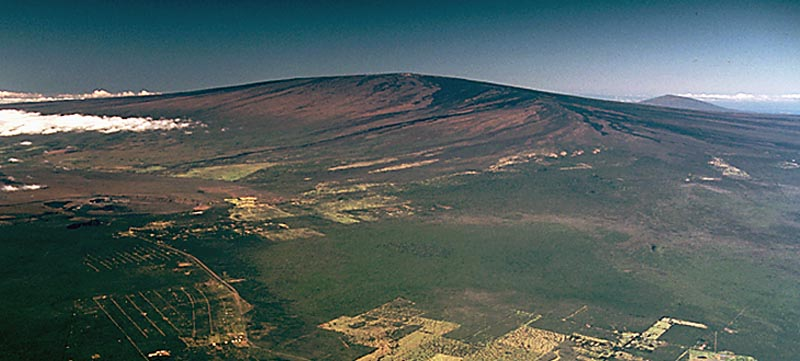
\includegraphics[width=0.8\linewidth]{images/book1/g7-mauna-loa.jpg}

{\small हवाई के बिग आइलैंड पर एक शील्ड \omterm{def:g4:volcanoes-earthquakes-first-look:volcano}{ज्वालामुखी}, मौना लोआ, हवा से: हल्की
ढलानों वाला एक विशाल पहाड़, जिसे पतले \omterm{def:g4:volcanoes-earthquakes-first-look:eruption}{लावा} के हज़ारों प्रवाहों ने बनाया है।
फ़ोटो: ग्रिग्स, अमेरिकी भूवैज्ञानिक सर्वेक्षण, 1985 (सार्वजनिक डोमेन,
विकिमीडिया कॉमन्स के ज़रिए)।}
% ledger: commons:mauna-loa
\label{fig:g7:volcanoes:mauna-loa}
\end{omfigure}

\section{ज्वालामुखियों के साथ जीना}

बहुत-से लोग \omterm{def:g4:volcanoes-earthquakes-first-look:volcano}{ज्वालामुखियों} के पास रहते हैं: 1991 में पिनातूबो के आसपास के
क्षेत्र में लगभग 3~मिलियन लोग रहते थे। सौभाग्य से, बड़ा \omterm{def:g4:volcanoes-earthquakes-first-look:eruption}{उद्गार} अक्सर चेतावनी
के संकेत देता है। ऊपर उठता \omterm{def:g7:volcanoes:magma}{मैग्मा} \omterm{def:g3:stones-pebbles-sand:rock}{चट्टानों} को किनारे धकेलता है: ज़मीन में दरारें
पड़ती हैं और वह छोटे \omterm{def:g4:volcanoes-earthquakes-first-look:earthquake}{भूकंपों} से काँपती है, ढलानें फूलती हैं, गैस निकलती है। माउंट
सेंट~हेलेंस पर पहले छोटे \omterm{def:g4:volcanoes-earthquakes-first-look:earthquake}{भूकंप} 16~मार्च 1980 को आए; 17~मई तक 10\,000 से
ज़्यादा आ चुके थे, और उत्तरी हिस्सा कम से कम \qty{137}{m} बाहर की ओर फूल चुका
था। वैज्ञानिकों ने यह सब मापा और क्षेत्र बंद कर दिया गया; फिर भी 18~मई को
57~लोग मारे गए।
% ledger: usgs:msh-lead-up, usgs:msh-flows

1991 में पिनातूबो पर, \omterm{def:g4:volcanoes-earthquakes-first-look:volcano}{ज्वालामुखी} के \omterm{def:g4:volcanoes-earthquakes-first-look:earthquake}{भूकंपों}, गैस और फूलने पर नज़र रखने वाले
वैज्ञानिकों ने समय रहते चेतावनी दे दी: \omterm{def:g4:volcanoes-earthquakes-first-look:volcano}{ज्वालामुखी} के पास रहने वाले लोग चले गए,
और कम से कम 5\,000 जानें बचाई गईं।
% ledger: usgs:pinatubo-1991 (central Luzon home to about 3 million people)

\begin{remark}[फटते ज्वालामुखी के पास कभी मत जाओ]\label{rem:g7:volcanoes:safety}
\omterm{def:g4:volcanoes-earthquakes-first-look:eruption}{उद्गार} देखना केवल उन जगहों से होता है जिन्हें अधिकारियों ने जनता के लिए खोला
है। गैसें, गिरती \omterm{def:g3:stones-pebbles-sand:rock}{चट्टानें}, पैरों के नीचे टूट जाने वाली \omterm{def:g4:volcanoes-earthquakes-first-look:eruption}{लावा} की ताज़ा परत और
\omterm{def:g7:volcanoes:pyroclastic-flow}{पायरोक्लास्टिक प्रवाह} जान ले सकते हैं, अक्सर बिना चेतावनी के। \omterm{def:g4:volcanoes-earthquakes-first-look:volcano}{ज्वालामुखी}
वेधशालाएँ बताती हैं कि कहाँ जाना सुरक्षित है: हमेशा उनकी बात मानो।
\end{remark}

\section{अभ्यास}

\begin{exercise}[$\star$]\label{exo:g7:volcanoes:1}
हर शब्द को उसके अर्थ से मिलाओ: \omterm{def:g7:volcanoes:magma}{मैग्मा}; \omterm{def:g4:volcanoes-earthquakes-first-look:eruption}{लावा}; \omterm{def:g7:volcanoes:magma-chamber}{मैग्मा कक्ष}; \omterm{def:g7:volcanoes:vent}{निकास-छिद्र};
\omterm{def:g7:volcanoes:vent}{क्रेटर}। (क) \omterm{def:g4:volcanoes-earthquakes-first-look:volcano}{ज्वालामुखी} की चोटी पर कटोरे के आकार का एक गड्ढा। (ख) ज़मीन के
नीचे की पिघली \omterm{def:g3:stones-pebbles-sand:rock}{चट्टान}। (ग) एक मुँह जिससे \omterm{def:g7:volcanoes:magma}{मैग्मा} बाहर आता है। (घ) सतह पर बाहर
आ चुकी पिघली \omterm{def:g3:stones-pebbles-sand:rock}{चट्टान}। (ङ) किसी \omterm{def:g4:volcanoes-earthquakes-first-look:volcano}{ज्वालामुखी} के कुछ किलोमीटर नीचे \omterm{def:g7:volcanoes:magma}{मैग्मा} की एक
बड़ी जेब।
\end{exercise}

\begin{exercise}[$\star$]\label{exo:g7:volcanoes:2}
बहिःस्रावी या विस्फोटक? (क) चमकते \omterm{def:g4:volcanoes-earthquakes-first-look:eruption}{लावा} की \omterm{def:g1:landscapes-around-us:water}{नदियाँ} एक हल्की ढलान से नीचे बहती
हैं। (ख) राख का एक स्तंभ आकाश में \qty{35}{km} ऊपर उठता है। (ग) एक दरार से
चमकती बूँदों का फव्वारा उछलता है। (घ) गरम राख और गैस का एक हिमस्खलन \omterm{def:g1:landscapes-around-us:landform}{घाटी} में
नीचे दौड़ता है।
\end{exercise}

\begin{exercise}[$\star$]\label{exo:g7:volcanoes:3}
सही या ग़लत? ग़लत वाक्यों को सुधारो। (क) \omterm{def:g7:volcanoes:magma}{मैग्मा} और \omterm{def:g4:volcanoes-earthquakes-first-look:eruption}{लावा} एक ही पिघली \omterm{def:g3:stones-pebbles-sand:rock}{चट्टान} के
दो नाम हैं, ज़मीन के नीचे और सतह पर। (ख) सबसे ज़्यादा मात्रा वाली \omterm{def:g4:volcanoes-earthquakes-first-look:volcano}{ज्वालामुखी}
गैस कार्बन डाइऑक्साइड है। (ग) \omterm{def:g7:volcanoes:pyroclastic-flow}{पायरोक्लास्टिक प्रवाह} द्रव \omterm{def:g4:volcanoes-earthquakes-first-look:eruption}{लावा} की एक \omterm{def:g1:landscapes-around-us:water}{नदी} है।
(घ) हवाई के \omterm{def:g4:volcanoes-earthquakes-first-look:volcano}{ज्वालामुखी} एक \omterm{def:g7:plate-tectonics:plate-boundary}{प्लेट सीमा} पर हैं।
\end{exercise}

\begin{exercise}[$\star$]\label{exo:g7:volcanoes:4}
चमक के रंगों वाली तालिका का उपयोग करो। (क) \omterm{def:g4:volcanoes-earthquakes-first-look:eruption}{लावा} पीला चमकता है: उसका तापमान
बताओ। (ख) सख़्त होता एक प्रवाह गहरा लाल चमकता है: उसका तापमान बताओ।
(ग) एक तस्वीर में प्रवाह के अगले सिरे पर नारंगी \omterm{def:g4:volcanoes-earthquakes-first-look:eruption}{लावा} और \omterm{def:g7:volcanoes:vent}{निकास-छिद्र} के पास पीला
\omterm{def:g4:volcanoes-earthquakes-first-look:eruption}{लावा} दिखता है। ज़्यादा गरम कहाँ है? क्यों?
\end{exercise}

\begin{exercise}[$\star\star$]\label{exo:g7:volcanoes:5}
1\,214 \omterm{def:g4:volcanoes-earthquakes-first-look:volcano}{ज्वालामुखियों} वाले दंड आलेख का उपयोग करो। (क) कितने \omterm{def:g4:volcanoes-earthquakes-first-look:volcano}{ज्वालामुखी} किसी
\omterm{def:g7:plate-tectonics:plate-boundary}{प्लेट सीमा} पर हैं (जहाँ \omterm{def:g7:plate-tectonics:plate}{प्लेटें} एक-दूसरे से दूर जाती हैं, या जहाँ एक दूसरी के
नीचे धँसती है)? (ख) यह सभी \omterm{def:g4:volcanoes-earthquakes-first-look:volcano}{ज्वालामुखियों} का कितना प्रतिशत है? (ग) जाँचो कि
प्रस्ताव के चारों प्रतिशतों का जोड़ लगभग 100~\% होता है।
\end{exercise}

\begin{exercise}[$\star\star$]\label{exo:g7:volcanoes:6}
सूची के 660 खड़े शंकुओं (स्तरित \omterm{def:g4:volcanoes-earthquakes-first-look:volcano}{ज्वालामुखियों}) में से 564 वहाँ हैं जहाँ एक \omterm{def:g7:plate-tectonics:plate}{प्लेट}
दूसरी के नीचे धँसती है, 62 वहाँ जहाँ \omterm{def:g7:plate-tectonics:plate}{प्लेटें} एक-दूसरे से दूर जाती हैं और 33 किसी
\omterm{def:g7:plate-tectonics:plate}{प्लेट} के अंदर। (क) उन खड़े शंकुओं का प्रतिशत निकालो जो वहाँ हैं जहाँ एक \omterm{def:g7:plate-tectonics:plate}{प्लेट}
दूसरी के नीचे धँसती है। (ख) ``ज्ञात नहीं'' स्थिति के लिए कितने खड़े शंकु बचते
हैं? (ग) चारों सुरागों का उपयोग करो: अग्नि-वलय के साथ-साथ हमें किस तरह के
\omterm{def:g4:volcanoes-earthquakes-first-look:eruption}{उद्गारों} की आशा करनी चाहिए?
\end{exercise}

\begin{exercise}[$\star\star$]\label{exo:g7:volcanoes:7}
किलाउआ पर \omterm{def:g4:volcanoes-earthquakes-first-look:eruption}{लावा} लगभग \qty{1170}{\degreeCelsius} पर \omterm{def:g7:volcanoes:vent}{निकास-छिद्र} से निकलता है।
एक \omterm{def:g4:volcanoes-earthquakes-first-look:eruption}{लावा} सुरंग में वह \qty{10}{km} दूर \omterm{def:g2:water-on-earth:ocean}{समुद्र} तक लगभग
\qty{1140}{\degreeCelsius} पर पहुँचा। (क) वह कितने डिग्री ठंडा हुआ? (ख) यह
प्रति किलोमीटर कितने डिग्री है? (ग) खुली हवा में \omterm{def:g4:volcanoes-earthquakes-first-look:eruption}{लावा} अपनी सतह पर प्रति सेकंड
सैकड़ों डिग्री ठंडा होता है। समझाओ कि सुरंग में \omterm{def:g4:volcanoes-earthquakes-first-look:eruption}{लावा} इतना गरम क्यों
रहा।
\end{exercise}

\begin{exercise}[$\star\star$]\label{exo:g7:volcanoes:8}
काउआई की सबसे पुरानी \omterm{def:g3:stones-pebbles-sand:rock}{चट्टानें} लगभग 5.5~मिलियन वर्ष पुरानी हैं; बिग आइलैंड की,
0.7~मिलियन वर्ष से कम पुरानी। (क) कौन-सा द्वीप ज़्यादा पुराना है? कम से कम
कितने मिलियन वर्ष? (ख) कौन-सा द्वीप ज़्यादा घिसा हुआ है? क्यों? (ग) आज कौन-सा
द्वीप \omterm{def:g7:volcanoes:hotspot}{तप्त स्थल} के ऊपर है? (घ) काउआई बिग आइलैंड के उत्तर-पश्चिम में है।
प्रशांत \omterm{def:g7:plate-tectonics:plate}{प्लेट} द्वीपों को किस दिशा में ले जाती
है?
\end{exercise}

\begin{exercise}[$\star\star$]\label{exo:g7:volcanoes:9}
हवाई के द्वीप सबसे पास वाली \omterm{def:g7:plate-tectonics:plate-boundary}{प्लेट सीमा} से \qty{3200}{km} से भी ज़्यादा दूर
हैं। (क) \omterm{def:g4:volcanoes-earthquakes-first-look:volcano}{ज्वालामुखियों} के लिए यह हैरानी की बात क्यों है? (ख) तीन या चार वाक्यों
में समझाओ कि उनका \omterm{def:g7:volcanoes:magma}{मैग्मा} कहाँ से आता है। (ग) \omterm{def:g4:volcanoes-earthquakes-first-look:volcano}{ज्वालामुखियों} के \omterm{def:g2:drawing-to-map:map}{मानचित्र} पर वे
किस रंग के हैं?
\end{exercise}

\begin{exercise}[$\star\star$]\label{exo:g7:volcanoes:10}
जून~1991 में पिनातूबो का पहला \omterm{def:g7:volcanoes:magma}{मैग्मा} शांति से रिसकर बाहर आया; तीन दिन बाद
दूसरा \omterm{def:g7:volcanoes:magma}{मैग्मा} फट पड़ा। सोडा वाटर की दो बोतलों की मदद से फ़र्क़ समझाओ। दोनों में
से किस \omterm{def:g7:volcanoes:magma}{मैग्मा} ने ऊपर आते हुए अपनी गैस खो दी थी?
\end{exercise}

\begin{exercise}[$\star\star\star$]\label{exo:g7:volcanoes:11}
एक गाँव एक \omterm{def:g4:volcanoes-earthquakes-first-look:volcano}{ज्वालामुखी} से \omterm{def:g1:landscapes-around-us:landform}{घाटी} में नीचे \qty{10}{km} दूर है। (क) एक
\omterm{def:g7:volcanoes:pyroclastic-flow}{पायरोक्लास्टिक प्रवाह} \qty{80}{km/h} की चाल से चलता है। उसे गाँव तक पहुँचने
में कितने मिनट लगेंगे? (ख) \qty{130}{km/h} पर यही प्रश्न। (ग) एक परिवार को
कार से निकलने में 20~मिनट लगते हैं। समझाओ कि चेतावनी \omterm{def:g4:volcanoes-earthquakes-first-look:eruption}{उद्गार} शुरू होने से पहले
क्यों आनी चाहिए, प्रवाह दिखने पर नहीं।
\end{exercise}

\begin{exercise}[$\star\star\star$]\label{exo:g7:volcanoes:12}
माउंट सेंट~हेलेंस की राख ने 15~दिनों में पूरी पृथ्वी का एक चक्कर लगाया।
\omterm{def:g6:latitude-longitude:latitude}{अक्षांश} का एक अंश लगभग \qty{111}{km} का होता है, और एक पूरा चक्कर 360~अंश का
है। (क) किलोमीटर में पृथ्वी का एक पूरा चक्कर लगभग कितना लंबा है? निकटतम हज़ार
तक पूर्णांकित करो। (ख) राख ने औसतन प्रति दिन कितने किलोमीटर यात्रा की? (ग) यह
प्रति घंटा कितने किलोमीटर है? (घ) राख को हवा ले जाती है या उसकी अपनी चाल?
समझाओ।
% ledger: usgs:msh-may18, rmg:latitude-def
\end{exercise}

\section{समस्या: वह दिन जब पहाड़ ने अपनी चोटी खो दी}

\begin{problem}[{सप्ताहांत समस्या --- माउंट सेंट~हेलेंस के चेतावनी संकेत,
18~मई 1980 का उद्गार, और पहाड़ का कितना हिस्सा ग़ायब हो गया}]
\label{pb:g7:volcanoes:1}
% ledger: usgs:msh-heights, usgs:msh-lead-up, usgs:msh-may18, usgs:msh-flows, usgs:msh-reach, usgs:msh-dome, usgs:msh-faq-loss, data:gvp, tht:everest

माउंट सेंट~हेलेंस संयुक्त राज्य अमेरिका के उत्तर-पश्चिम में है। अध्याय की शुरुआत
की तस्वीरों, \omterm{def:g4:volcanoes-earthquakes-first-look:volcano}{ज्वालामुखियों} के \omterm{def:g2:drawing-to-map:map}{मानचित्र} और अमेरिकी भूवैज्ञानिक सर्वेक्षण द्वारा मापी
गई नीचे की संख्याओं का उपयोग करो।

\medskip
\noindent\textbf{भाग I --- उद्गार से पहले।}
\begin{enumerate}
  \item पहले छोटे \omterm{def:g4:volcanoes-earthquakes-first-look:earthquake}{भूकंप} 16~मार्च 1980 को आए; बड़ा \omterm{def:g4:volcanoes-earthquakes-first-look:eruption}{उद्गार} 18~मई को। दोनों के बीच
        कितने दिन बीते? (मार्च में 31~दिन होते हैं, अप्रैल
        में~30।)
  \item 17~मई तक, 16~मार्च के बाद के 62~दिनों में, 10\,000 से ज़्यादा \omterm{def:g4:volcanoes-earthquakes-first-look:earthquake}{भूकंप}
        दर्ज हो चुके थे। यह औसतन प्रति दिन लगभग कितने
        हैं?
  \item पहाड़ का उत्तरी हिस्सा कम से कम \qty{137}{m} बाहर की ओर फूल गया। समझाओ
        कि इस फूलने से वैज्ञानिक चिंतित क्यों हुए।
  \item \omterm{def:g4:volcanoes-earthquakes-first-look:volcano}{ज्वालामुखियों} के \omterm{def:g2:drawing-to-map:map}{मानचित्र} पर माउंट सेंट~हेलेंस एक नीला त्रिकोण है। इससे
        उसकी स्थिति के बारे में क्या पता चलता है? तुम किस तरह के \omterm{def:g4:volcanoes-earthquakes-first-look:eruption}{उद्गार} की आशा
        करते हो, और \omterm{def:g4:volcanoes-earthquakes-first-look:volcano}{ज्वालामुखी} के किस आकार की?
\end{enumerate}

\medskip
\noindent\textbf{भाग II --- 18 मई 1980।}\par\nopagebreak
\begin{enumerate}[resume, beginpenalty=10000]
  \item सुबह 8:32 बजे एक छोटे \omterm{def:g4:volcanoes-earthquakes-first-look:earthquake}{भूकंप} ने फूले हुए हिस्से को फिसला दिया। \omterm{def:g5:natural-hazards:landslide}{भूस्खलन}
        \qty{240}{km/h} तक की चाल से चला। यह प्रति मिनट कितने
        किलोमीटर है?
  \item \omterm{def:g5:natural-hazards:landslide}{भूस्खलन} ने \omterm{def:g7:volcanoes:magma}{मैग्मा} को वैसे ही खोल दिया जैसे हिलाई हुई बोतल से कॉर्क खींच
        लिया जाए। समझाओ कि फिर \omterm{def:g4:volcanoes-earthquakes-first-look:volcano}{ज्वालामुखी} एक तरफ़ को क्यों फटा।
  \item एक तरफ़ को हुआ विस्फोट कम से कम \qty{480}{km/h} की चाल से चला और
        \omterm{def:g4:volcanoes-earthquakes-first-look:volcano}{ज्वालामुखी} से \qty{27}{km} तक पहुँचा। उस चाल से वहाँ पहुँचने में उसे
        ज़्यादा से ज़्यादा कितने मिनट लगे?
  \item \omterm{def:g7:volcanoes:pyroclastic-flow}{पायरोक्लास्टिक प्रवाह} \qty{130}{km/h} तक की चाल से चले और \omterm{def:g7:volcanoes:vent}{क्रेटर} से
        \qty{8}{km} तक पहुँचे। उस चाल से उन्हें कितने मिनट लगे? निकटतम मिनट तक
        पूर्णांकित करो।
\end{enumerate}

\medskip
\noindent\textbf{भाग III --- बाद में।}\par\nopagebreak
\begin{enumerate}[resume, beginpenalty=10000]
  \item राख का स्तंभ 15~मिनट से कम में लगभग \qty{24}{km} की ऊँचाई तक पहुँचा।
        यह माउंट एवरेस्ट (\qty{8.8}{km}) से कितने गुना ऊँचा है? एक दशमलव स्थान
        तक पूर्णांकित करो।
  \item 1980 और 1986 के बीच \omterm{def:g7:volcanoes:vent}{क्रेटर} में चिपचिपा \omterm{def:g4:volcanoes-earthquakes-first-look:eruption}{लावा} रिसकर निकला और
        \omterm{def:g7:volcanoes:vent}{निकास-छिद्र} के ऊपर \qty{267}{m} ऊँचा एक टीला बना दिया। ये \omterm{def:g4:volcanoes-earthquakes-first-look:eruption}{उद्गार}
        बहिःस्रावी थे या विस्फोटक? ये तुम्हें सोडा वाटर की किस बोतल की याद
        दिलाते हैं?
  \item \omterm{def:g4:volcanoes-earthquakes-first-look:volcano}{ज्वालामुखी} की दोनों तस्वीरें देखो। दो वाक्यों में बताओ कि क्या
        बदला।
  \item \omterm{def:g4:volcanoes-earthquakes-first-look:eruption}{उद्गार} से पहले चोटी \omterm{def:g4:world-physical-map:altitude}{समुद्र तल} से \qty{2950}{m} ऊपर थी; उसके बाद सबसे
        ऊँचा बिंदु \qty{2549}{m} पर था। पहाड़ ने कितने मीटर ऊँचाई
        खोई?
\end{enumerate}
\end{problem}
